% questions.tex —— 2020 年·新高考Ⅱ卷 · 题目内容片段（无答案）
% 由 tools/generate_projects.py 依来源总账自 2020/2020_数学真题_新高考Ⅱ_试题.md 生成，勿手改（改源 MD 后重跑）


\begin{gknotice}
\textbf{结构提示}：本卷为 \textbf{22 题制}（2024 年起改为 19 题制），宜按知识点抽题使用，不宜整套限时模拟。

\textbf{卷种说明}：2020 年为新高考首批试点年份，本卷（新高考 Ⅱ 卷）由海南使用。

\textbf{适用省份}：海南
\end{gknotice}

\par\medskip

\gkpart{一、单选题}

\begin{gktip}
本题共 8 小题，每小题 5 分，共 40 分。在每小题给出的四个选项中，只有一项是符合题目要求的。
\end{gktip}

\begin{question}
\gkti{1}设集合 $A=\{2,3,5,7\}$，$B=\{1,2,3,5,8\}$，则 $A\cap B=$\mbox{（　　）}

\begin{gkopts}(4)
\task A．$\{1,8\}$
\task B．$\{2,5\}$
\task C．$\{2,3,5\}$
\task D．$\{1,2,3,5,8\}$
\end{gkopts}

\end{question}
\begin{question}
\gkti{2}$(1+2\mathrm i)(2+\mathrm i)=$\mbox{（　　）}

\begin{gkopts}(4)
\task A．$-5\mathrm i$
\task B．$5\mathrm i$
\task C．$-5$
\task D．$5$
\end{gkopts}

\end{question}
\begin{question}
\gkti{3}若 $D$ 为 $\triangle ABC$ 的边 $AB$ 的中点，则 $\overrightarrow{CB}=$\mbox{（　　）}

\begin{gkopts}(2)
\task A．$2\overrightarrow{CD}-\overrightarrow{CA}$
\task B．$2\overrightarrow{CA}-\overrightarrow{CD}$
\task C．$2\overrightarrow{CD}+\overrightarrow{CA}$
\task D．$2\overrightarrow{CA}+\overrightarrow{CD}$
\end{gkopts}

\end{question}
\begin{question}
\gkti{4}日晷是中国古代用来测定时间的仪器，利用与晷面垂直的晷针投射到晷面的影子来测定时间。把地球看成一个球（球心记为 $O$），地球上一点 $A$ 的纬度是指 $OA$ 与地球赤道所在平面所成角，点 $A$ 处的水平面是指过点 $A$ 且与 $OA$ 垂直的平面。在点 $A$ 处放置一个日晷，若晷面与赤道所在平面平行，点 $A$ 处的纬度为北纬 $40^\circ$，则晷针与点 $A$ 处的水平面所成角为\mbox{（　　）}

\begin{gkopts}(4)
\task A．$20^\circ$
\task B．$40^\circ$
\task C．$50^\circ$
\task D．$90^\circ$
\end{gkopts}

\end{question}
\begin{question}
\gkti{5}某中学的学生积极参加体育锻炼，其中有 $96\%$ 的学生喜欢足球或游泳，$60\%$ 的学生喜欢足球，$82\%$ 的学生喜欢游泳，则该中学既喜欢足球又喜欢游泳的学生数占该校学生总数的比例是\mbox{（　　）}

\begin{gkopts}(4)
\task A．$62\%$
\task B．$56\%$
\task C．$46\%$
\task D．$42\%$
\end{gkopts}

\end{question}
\begin{question}
\gkti{6}$3$ 名大学生利用假期到 $2$ 个山村参加扶贫工作，每名大学生只去 $1$ 个村，每个村至少 $1$ 人，则不同的分配方案共有\mbox{（　　）}

\begin{gkopts}(4)
\task A．$4$ 种
\task B．$5$ 种
\task C．$6$ 种
\task D．$8$ 种
\end{gkopts}

\end{question}
\begin{question}
\gkti{7}已知函数 $f(x)=\lg\left(x^{2}-4x-5\right)$ 在 $(a,+\infty)$ 单调递增，则 $a$ 的取值范围是\mbox{（　　）}

\begin{gkopts}(4)
\task A．$(-\infty,-1]$
\task B．$(-\infty,2]$
\task C．$[2,+\infty)$
\task D．$[5,+\infty)$
\end{gkopts}

\end{question}
\begin{question}
\gkti{8}若定义在 $\mathbf R$ 的奇函数 $f(x)$ 在 $(-\infty,0)$ 单调递减，且 $f(2)=0$，则满足 $xf(x-1)\ge0$ 的 $x$ 的取值范围是\mbox{（　　）}

\begin{gkopts}(2)
\task A．$[-1,1]\cup[3,+\infty)$
\task B．$[-3,-1]\cup[0,1]$
\task C．$[-1,0]\cup[1,+\infty)$
\task D．$[-1,0]\cup[1,3]$
\end{gkopts}

\par\medskip

\end{question}
\gkpart{二、多选题}

\begin{gktip}
本题共 4 小题，每小题 5 分，共 20 分。全部选对得 5 分，部分选对得 2 分，有选错得 0 分。
\end{gktip}

\Needspace{0.4\textheight}
\begin{question}
\gkti{9}我国新冠肺炎疫情进入常态化，各地有序推进复工复产，下面是某地连续 $11$ 天复工复产指数折线图，下列说法正确的是\mbox{（　　）}
\nopagebreak[4]
\begin{center}% 2020 新高考Ⅱ卷 9：某地区复工复产指数折线图（连续 11 天）
% 绘制依据：源 PDF 原图逐点核对。横轴「天数」等距标 1–11；纵轴「指数」不从 0 起，
% 只画 78%/80%/82% 三条水平虚线并在左侧标注；右上角图例：空心圆＝复产指数，实心圆＝复工指数。
% 必须保住的形态：第 2 天复工为全图最低且恰在 78% 线上；第 6 天复工恰在 82% 线上；
% 第 3 天起两线均在 80% 线上方；第 8→9 天两线交叉，其后复工在上（第 11 天复产重新略高）；
% 第 1 天两线间距明显大于第 11 天。
% 说明：第 2 天复工取 78.0、第 6 天复工取 82.0（转录读数 77.9 / 82.1），
% 以保住原图「恰落在虚线上」的定性特征——0.1 的差在本图尺度上会明显浮出虚线。
\begin{tikzpicture}
\begin{axis}[width=10.6cm, height=6.4cm, font=\small,
  axis lines=left,
  xlabel={天数}, ylabel={指数},
  xlabel style={at={(1,0)}, anchor=north west},
  ylabel style={at={(0,1)}, anchor=south, rotate=-90},
  xmin=0.35, xmax=11.75, ymin=76.9, ymax=87.4,
  xtick={1,2,...,11},
  ytick={78,80,82},
  yticklabels={$78\%$,$80\%$,$82\%$},
  ymajorgrids=true, grid style={dashed, gray!65},
  legend cell align=left,
  legend style={at={(0.995,0.99)}, anchor=north east, draw=none, fill=white,
                font=\small, row sep=-2pt, inner sep=2pt}]
  \addplot[thick, mark=o, mark size=1.7pt, mark options={fill=white}]
    coordinates {(1,80.6) (2,80.8) (3,81.6) (4,82.4) (5,82.6) (6,83.0)
                 (7,84.0) (8,83.4) (9,81.6) (10,82.8) (11,84.4)};
  \addlegendentry{复产指数}
  \addplot[thick, mark=*, mark size=1.7pt]
    coordinates {(1,79.7) (2,78.0) (3,80.5) (4,81.1) (5,81.3) (6,82.0)
                 (7,82.3) (8,81.7) (9,83.2) (10,84.5) (11,83.9)};
  \addlegendentry{复工指数}
\end{axis}
\end{tikzpicture}
\end{center}
\nopagebreak[4]
\begin{gkopts}(1)
\task A．这 $11$ 天复工指数和复产指数均逐日增加
\task B．这 $11$ 天期间，复产指数增量大于复工指数的增量
\task C．第 $3$ 天至第 $11$ 天复工复产指数均超过 $80\%$
\task D．第 $9$ 天至第 $11$ 天复产指数增量大于复工指数的增量
\end{gkopts}

\end{question}
\begin{question}
\gkti{10}已知曲线 $C:mx^{2}+ny^{2}=1$\mbox{（　　）}

\begin{gkopts}(1)
\task A．若 $m>n>0$，则 $C$ 是椭圆，其焦点在 $y$ 轴上
\task B．若 $m=n>0$，则 $C$ 是圆，其半径为 $\sqrt n$
\task C．若 $mn<0$，则 $C$ 是双曲线，其渐近线方程为 $y=\pm\sqrt{-\dfrac mn}\,x$
\task D．若 $m=0$，$n>0$，则 $C$ 是两条直线
\end{gkopts}

\Needspace{0.4\textheight}
\end{question}
\begin{question}
\gkti{11}下图是函数 $y=\sin(\omega x+\varphi)$ 的部分图象，则 $\sin(\omega x+\varphi)=$\mbox{（　　）}
\nopagebreak[4]
\begin{center}% 2020 新高考Ⅱ卷 11：正弦型函数 y=sin(2x+2π/3) 的图象，x∈[−π/3, 7π/6]
% 绘制依据：源 PDF 原图。形态锚点：最大值在 x=−π/12（y 轴稍左）、x=π/6 处下穿 x 轴、
% 最小值 x=5π/12、x=2π/3 处上穿、x=11π/12 再现波峰；区间两端恰为零点（跨 1.5 个周期）。
% y 轴只标刻度 1（置于 (0,1) 左上方以避开紧邻 y 轴的波峰）；
% x 轴只标 π/6 与 2π/3，用手工节点分置左下 / 右下以避让曲线；O 标原点左下。
\begin{tikzpicture}
\begin{axis}[width=10.6cm, height=5.6cm, font=\small,
  axis lines=middle, xlabel={$x$}, ylabel={$y$},
  xmin=-1.35, xmax=4.05, ymin=-1.45, ymax=1.62,
  xtick=\empty, ytick=\empty,
  every axis x label/.style={at={(current axis.right of origin)}, anchor=west},
  every axis y label/.style={at={(current axis.above origin)}, anchor=south}]
  \addplot[domain=-1.0472:3.6652, samples=250, thick] {sin(deg(2*x+2*pi/3))};
  \draw (axis cs:-0.06,1) -- (axis cs:0.06,1);
  \node[above left, inner sep=1pt] at (axis cs:0,1) {$1$};
  \node[below left, inner sep=1pt] at (axis cs:0.5236,0) {$\frac{\pi}{6}$};
  \node[below right, inner sep=1pt] at (axis cs:2.0944,0) {$\frac{2\pi}{3}$};
  \node[below left, inner sep=1pt] at (axis cs:0,0) {$O$};
\end{axis}
\end{tikzpicture}
\end{center}
\nopagebreak[4]
\begin{gkopts}(2)
\task A．$\sin\left(x+\dfrac\pi3\right)$
\task B．$\sin\left(\dfrac\pi3-2x\right)$
\task C．$\cos\left(2x+\dfrac\pi6\right)$
\task D．$\cos\left(\dfrac{5\pi}6-2x\right)$
\end{gkopts}

\end{question}
\begin{question}
\gkti{12}已知 $a>0$，$b>0$，且 $a+b=1$，则\mbox{（　　）}

\begin{gkopts}(2)
\task A．$a^{2}+b^{2}\ge\dfrac12$
\task B．$2^{a-b}>\dfrac12$
\task C．$\log_2a+\log_2b\ge-2$
\task D．$\sqrt a+\sqrt b\le\sqrt2$
\end{gkopts}

\par\medskip

\end{question}
\gkpart{三、填空题}

\begin{gktip}
本题共 4 小题，每小题 5 分，共 20 分。
\end{gktip}

\begin{question}
\gkti{13}棱长为 $2$ 的正方体 $ABCD\text{-}A_1B_1C_1D_1$ 中，$M$，$N$ 分别为棱 $BB_1$，$AB$ 的中点，则三棱锥 $A\text{-}NMD_1$ 的体积为 \gkblank{}．

\end{question}
\begin{question}
\gkti{14}斜率为 $\sqrt3$ 的直线过抛物线 $C:y^{2}=4x$ 的焦点，且与 $C$ 交于 $A$，$B$ 两点，则 $|AB|=$ \gkblank{}．

\end{question}
\begin{question}
\gkti{15}将数列 $\{2n-1\}$ 与 $\{3n-2\}$ 的公共项从小到大排列得到数列 $\left\{a_n\right\}$，则 $\left\{a_n\right\}$ 的前 $n$ 项和为 \gkblank{}．

\Needspace{0.4\textheight}
\end{question}
\begin{question}
\gkti{16}某中学开展劳动实习，学生加工制作零件，零件的截面如图所示。$O$ 为圆孔及轮廓圆弧 $AB$ 所在圆的圆心，$A$ 是圆弧 $AB$ 与直线 $AG$ 的切点，$B$ 是圆弧 $AB$ 与直线 $BC$ 的切点，四边形 $DEFG$ 为矩形，$BC\perp DG$，垂足为 $C$，$\tan\angle ODC=\dfrac35$，$BH\parallel DG$，$EF=12\ \mathrm{cm}$，$DE=2\ \mathrm{cm}$，$A$ 到直线 $DE$ 和 $EF$ 的距离均为 $7\ \mathrm{cm}$，圆孔半径为 $1\ \mathrm{cm}$，则图中阴影部分的面积为 \gkblank{} $\mathrm{cm}^{2}$．
\nopagebreak[4]
\begin{center}% 2020 新高考Ⅱ卷 16：某零件的截面（1 单位 = 1 cm，整图 scale=0.75）
% 绘制依据：源 PDF 原图逐像素核对。矩形 DEFG：D(0,2)、E(0,0)、F(12,0)、G(12,2)，
% ED/EF/FG 实线、DG 虚线；外轮廓弧圆心 O(5,5)、半径 R=2√2，弧顶 (5,7.83)；
% A(7,7) 与 B(2.172,5) 为切点（GA 与弧相切于 A、竖直的 BC 与弧相切于 B），
% C(2.172,2) 是 B 在 DG 上的垂足，H(9,5) 在直线 GA 上且与 B、O 共线于 y=5。
% 实线闭合轮廓：E→F→G→A→（弧 45°逆时针经弧顶到 180°）→B→C→D→E。
% 虚线四条：B–O–H、D–C…G、过 O 的竖直中心线（弧顶落到 (5,2)）、线段 D–O。
% 阴影 gray!25：弧 B→A + 线段 A→H + 线段 H→B 围成的区域；半径 1 的圆孔整体留白
% （先填灰、再以白色填圆，故 BH 以下不着色），中心线穿孔而过。
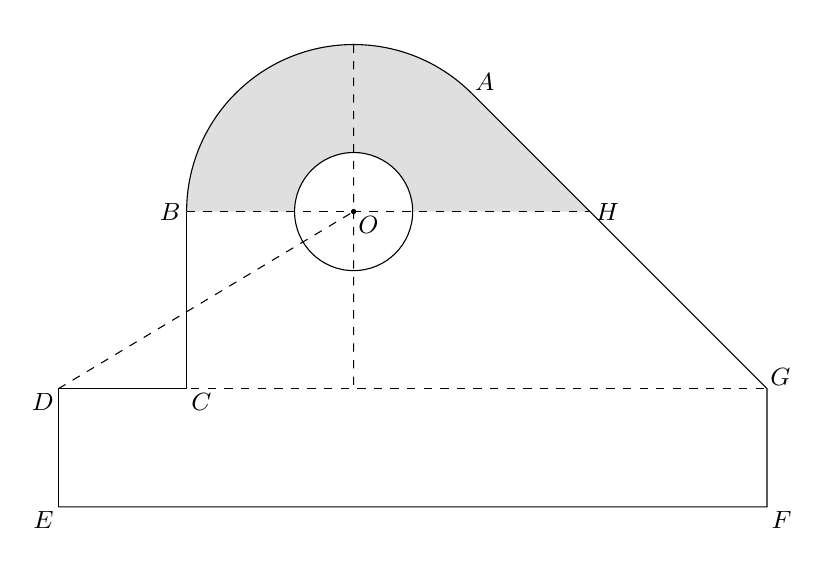
\begin{tikzpicture}[scale=0.75, font=\small]
  \coordinate (D) at (0,2);
  \coordinate (E) at (0,0);
  \coordinate (F) at (12,0);
  \coordinate (G) at (12,2);
  \coordinate (O) at (5,5);
  \coordinate (A) at (7,7);
  \coordinate (B) at (2.1716,5);
  \coordinate (C) at (2.1716,2);
  \coordinate (H) at (9,5);
  \coordinate (T) at (5,7.8284);
  % ---------- 阴影：弧 B→A + AH + HB，随后把圆孔填白 ----------
  \fill[gray!25] (B) arc[start angle=180, end angle=45, radius=2.8284] -- (H) -- cycle;
  \fill[white] (O) circle (1);
  % ---------- 虚线 ----------
  \draw[dashed] (B) -- (H);
  \draw[dashed] (D) -- (G);
  \draw[dashed] (T) -- (5,2);
  \draw[dashed] (D) -- (O);
  % ---------- 实线轮廓与圆孔 ----------
  \draw (E) -- (F) -- (G) -- (A);
  \draw (A) arc[start angle=45, end angle=180, radius=2.8284];
  \draw (B) -- (C) -- (D) -- (E);
  \draw (O) circle (1);
  \fill (O) circle (1.3pt);
  % ---------- 标签 ----------
  \node[above right, inner sep=1pt] at (A) {$A$};
  \node[left, inner sep=2pt] at (B) {$B$};
  \node[below right, inner sep=1.5pt] at (C) {$C$};
  \node[below left, inner sep=1.5pt] at (D) {$D$};
  \node[below left, inner sep=1.5pt] at (E) {$E$};
  \node[below right, inner sep=1.5pt] at (F) {$F$};
  \node[above right, inner sep=1pt] at (G) {$G$};
  \node[right, inner sep=2pt] at (H) {$H$};
  \node[below right, inner sep=1.5pt] at (O) {$O$};
\end{tikzpicture}
\end{center}
\nopagebreak[4]
\par\medskip

\end{question}
\gkpart{四、解答题}

\begin{gktip}
本题共 6 小题，共 70 分。解答应写出文字说明、证明过程或演算步骤。
\end{gktip}

\begin{question}
\gkti{17}\textbf{（10 分）} 在① $ac=\sqrt3$，② $c\sin A=3$，③ $c=\sqrt3b$ 这三个条件中任选一个，补充在下面问题中，若问题中的三角形存在，求 $c$ 的值；若问题中的三角形不存在，说明理由。

问题：是否存在 $\triangle ABC$，它的内角 $A$，$B$，$C$ 的对边分别为 $a$，$b$，$c$，且 $\sin A=\sqrt3\sin B$，$C=\dfrac\pi6$，\gkblank{}？

\end{question}
\begin{question}
\gkti{18}\textbf{（12 分）} 已知公比大于 $1$ 的等比数列 $\left\{a_n\right\}$ 满足 $a_2+a_4=20$，$a_3=8$。

  (1) 求 $\left\{a_n\right\}$ 的通项公式；

  (2) 求 $a_1a_2-a_2a_3+\cdots+(-1)^{n-1}a_na_{n+1}$。

\end{question}
\begin{question}
\gkti{19}\textbf{（12 分）} 为加强环境保护，治理空气污染，环境监测部门对某市空气质量进行调研，随机抽查了 $100$ 天空气中的 PM2.5 和 $\mathrm{SO_2}$ 浓度（单位：$\mu\mathrm g/\mathrm m^{3}$），得下表：

\begin{center}
\begin{tabular}{cccc}
\toprule
$\mathrm{SO_2}$ 浓度 & $[0,50]$ & $(50,150]$ & $(150,475]$ \\
\midrule
PM2.5 $[0,35]$ & $32$ & $18$ & $4$ \\
PM2.5 $(35,75]$ & $6$ & $8$ & $12$ \\
PM2.5 $(75,115]$ & $3$ & $7$ & $10$ \\
\bottomrule
\end{tabular}
\end{center}

  (1) 估计事件"该市一天空气中 PM2.5 浓度不超过 $75$，且 $\mathrm{SO_2}$ 浓度不超过 $150$"的概率；

  (2) 根据所给数据，完成下面的 $2\times2$ 列联表：

\begin{center}
\begin{tabular}{ccc}
\toprule
$\mathrm{SO_2}$ 浓度 & $[0,150]$ & $(150,475]$ \\
\midrule
PM2.5 $[0,75]$ &  &  \\
PM2.5 $(75,115]$ &  &  \\
\bottomrule
\end{tabular}
\end{center}

  (3) 根据 (2) 中的列联表，判断是否有 $99\%$ 的把握认为该市一天空气中 PM2.5 浓度与 $\mathrm{SO_2}$ 浓度有关？

\Needspace{10\baselineskip}
  附：$K^{2}=\dfrac{n(ad-bc)^{2}}{(a+b)(c+d)(a+c)(b+d)}$

\begin{center}
\begin{tabular}{cccc}
\toprule
$P\left(K^{2}\ge k\right)$ & $0.050$ & $0.010$ & $0.001$ \\
\midrule
$k$ & $3.841$ & $6.635$ & $10.828$ \\
\bottomrule
\end{tabular}
\end{center}

\Needspace{0.4\textheight}
\end{question}
\begin{question}
\gkti{20}\textbf{（12 分）} 如图，四棱锥 $P\text{-}ABCD$ 的底面为正方形，$PD\perp$ 底面 $ABCD$。设平面 $PAD$ 与平面 $PBC$ 的交线为 $l$。
\nopagebreak[4]
\begin{center}% 2020 新高考Ⅱ卷 20：四棱锥 P-ABCD（底面 ABCD 为正方形，PD⊥底面 ABCD）
% 绘制依据：源 PDF 原图。底面按斜二测画：A 左前、B 右前、C 右后、D 中后（被遮挡顶点）；
% PD 垂直底面，故 P 画在 D 的正上方（位于版面中偏左）。
% 实线：PA、PB、PC、AB、BC；虚线：PD、AD、DC。只标 P、A、B、C、D 五点。
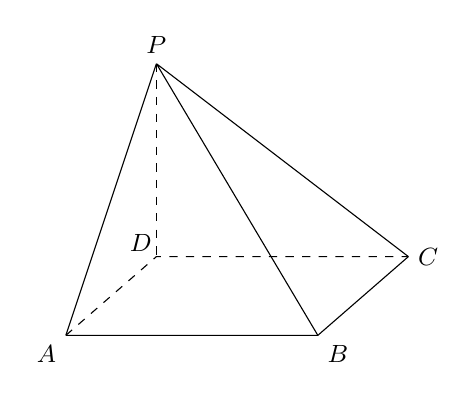
\begin{tikzpicture}[scale=1.0, font=\small]
  \coordinate (A) at (0,0);
  \coordinate (B) at (3.2,0);
  \coordinate (C) at (4.35,1.0);
  \coordinate (D) at (1.15,1.0);
  \coordinate (P) at (1.15,3.45);
  \draw (P) -- (A)  (P) -- (B)  (P) -- (C);
  \draw (A) -- (B) -- (C);
  \draw[dashed] (P) -- (D);
  \draw[dashed] (A) -- (D) -- (C);
  \node[above] at (P) {$P$};
  \node[below left] at (A) {$A$};
  \node[below right] at (B) {$B$};
  \node[right] at (C) {$C$};
  \node[above left, inner sep=1.5pt] at (D) {$D$};
\end{tikzpicture}
\end{center}
\nopagebreak[4]
  (1) 证明：$l\perp$ 平面 $PDC$；

  (2) 已知 $PD=AD=1$，$Q$ 为 $l$ 上的点，$QB=\sqrt2$，求 $PB$ 与平面 $QCD$ 所成角的正弦值。

\end{question}
\begin{question}
\gkti{21}\textbf{（12 分）} 已知椭圆 $C:\dfrac{x^{2}}{a^{2}}+\dfrac{y^{2}}{b^{2}}=1\ (a>b>0)$ 过点 $M(2,3)$，点 $A$ 为其左顶点，且 $AM$ 的斜率为 $\dfrac12$。

  (1) 求 $C$ 方程；

  (2) 点 $N$ 为椭圆上任意一点，求 $\triangle AMN$ 的面积的最大值。

\end{question}
\begin{question}
\gkti{22}\textbf{（12 分）} 已知函数 $f(x)=a\mathrm e^{x-1}-\ln x+\ln a$。

  (1) 当 $a=\mathrm e$ 时，求曲线 $y=f(x)$ 在点 $(1,f(1))$ 处的切线与两坐标轴围成的三角形的面积；

  (2) 若 $f(x)\ge1$，求 $a$ 的取值范围。

\par\medskip

\begin{gktip}
\textbf{试题来源}：deekur/gaokaomath（commit \texttt{34c13a6}，CC BY 4.0）之「2020新高考2(海南)」PDF。
\end{gktip}

\end{question}